\documentclass[11pt,a4paper]{article}

% --------------------------------------------------
% Packages
% --------------------------------------------------
\usepackage[T1]{fontenc}
\usepackage[utf8]{inputenc}
\usepackage{lmodern}
\usepackage[margin=2.5cm]{geometry}
\usepackage{microtype}

\usepackage{amsmath,amssymb}
\usepackage{graphicx}
\usepackage[numbers]{natbib}
\usepackage{booktabs}
\usepackage{caption}
\usepackage{hyperref}

% --------------------------------------------------
% Formatting
% --------------------------------------------------
\hypersetup{hidelinks}
\captionsetup{font=small,labelfont=bf}

% --------------------------------------------------
% Title
% --------------------------------------------------
\title{\textbf{Calibration of Regional Demand Slopes and Supply-Side Cost Parameters}}
\author{Alexander Csekö}
\date{March 2026}

\begin{document}

\maketitle

\section{Demand Calibration}

Regional module willingness-to-pay is derived from an LCOE-parity approach:
\begin{equation}
WTP_i^{sys} = \frac{\pi_{e,i} \cdot CF_i \cdot 8760}{CRF(r,L)},
\end{equation}
with
\begin{equation}
CRF(r,L) = \frac{r(1+r)^L}{(1+r)^L - 1}.
\end{equation}

Module-specific willingness-to-pay is then calculated as
\begin{equation}
WTP_i = s_{mod} \cdot WTP_i^{sys},
\end{equation}
where $s_{mod}=0.40$.

The 2025 slope of the linear demand function is calibrated using a point-elasticity approach:
\begin{equation}
b_{2025,i} = -\epsilon \cdot \frac{Dmax_{2025,i}}{WTP_i},
\end{equation}
for elasticity assumptions $\epsilon \in \{-0.65,-0.90,-1.20\}$.

\begin{table}[ht]
\centering
\caption{Regional maximum willingness-to-pay ($WTP_i$) and derived 2025 demand slopes ($b_{2025,i}$).}
\label{tab:wtp_and_slopes}
\begin{tabular}{lrrrrrrr}
\toprule
& & & & & \multicolumn{3}{c}{$b_{2025,i}$ [GW/\$]} \\
\cmidrule(lr){6-8}
\textbf{Region} &
\textbf{$\pi_{e,i}$ [\$/kWh]} &
\textbf{$CF_i$ [-]} &
\textbf{$WTP_i^{sys}$ [\$/kW]} &
\textbf{$WTP_i$ [\$/kW]} &
\textbf{Low} &
\textbf{Base} &
\textbf{High} \\
\midrule
ch   & 0.082 & 0.17 & 1303.54 & 521.42  & 0.347 & 0.480 & 0.640 \\
eu   & 0.199 & 0.13 & 2419.13 & 967.65  & 0.040 & 0.055 & 0.073 \\
us   & 0.075 & 0.20 & 1402.67 & 561.07  & 0.044 & 0.061 & 0.082 \\
apac & 0.084 & 0.17 & 1335.34 & 534.14  & 0.060 & 0.083 & 0.110 \\
af   & 0.138 & 0.22 & 2839.00 & 1135.60 & 0.010 & 0.014 & 0.019 \\
row  & 0.162 & 0.16 & 2423.81 & 969.52  & 0.019 & 0.026 & 0.034 \\
\bottomrule
\end{tabular}

\vspace{0.6em}
\footnotesize
Notes: $WTP_i^{sys}$ denotes the maximum allowable CAPEX for the full PV system. Module willingness-to-pay is calculated as $WTP_i = 0.40 \cdot WTP_i^{sys}$. Demand slopes are computed as $b_{2025,i} = -\epsilon \cdot (Dmax_{2025,i}/WTP_i)$.
\end{table}

\subsection*{Sources and Assumptions}
\begin{itemize}
    \item \textbf{Module cost share ($s_{mod}=0.40$):} based on utility-scale PV cost breakdowns reported by IRENA \cite{irena_cost_2024}.
    \item \textbf{Discount rate and lifetime ($r=8\%$, $L=25$):} stylized assumptions informed by NREL ATB methodology \cite{nrel_atb_2024}.
    \item \textbf{Capacity factors ($CF_i$):} based on PV yield data from the Global Solar Atlas \cite{globalsolaratlas}.
    \item \textbf{Electricity prices ($\pi_{e,i}$):} stylized regional benchmark values informed by the IEA World Energy Outlook \cite{iea_weo_2024}.
    \item \textbf{Elasticity range ($\epsilon \in [-1.20,-0.65]$):} chosen to span plausible responsiveness cases based on empirical literature \cite{gillingham_2018,hughes_2015}.
\end{itemize}






\subsection{Calibration of Inverse Demand Parameters}

Demand in each region \(i\) and year \(t\) is represented by the inverse demand function
\begin{equation}
\lambda_{i,t} = a_{i,s} - b_{i,t,s}\,q_{i,t},
\label{eq:inverse_demand}
\end{equation}
where \(q_{i,t}\) denotes served demand, \(\lambda_{i,t}\) the endogenous market price, and \(s\) the elasticity scenario. The associated quadratic utility function in the lower-level problem is
\begin{equation}
U_{i,t}(q_{i,t}) = a_{i,s}q_{i,t} - \frac{1}{2} b_{i,t,s} q_{i,t}^2,
\end{equation}
subject to
\begin{equation}
0 \le q_{i,t} \le D^{\max}_{i,t}.
\end{equation}

\paragraph{Assumptions.}
The calibration is based on the following assumptions:
\begin{itemize}
    \item The previously derived regional willingness-to-pay is interpreted as the full-demand threshold price,
    \begin{equation}
    p_i^{full} \equiv WTP_i.
    \end{equation}
    Thus, full demand is still served at price \(WTP_i\).
    
    \item Demand is capped by the exogenous market size \(D^{\max}_{i,t}\).
    
    \item The elasticity is imposed at the calibration point \(\bigl(q_{i,t},\lambda_{i,t}\bigr)=\bigl(D^{\max}_{i,t},WTP_i\bigr)\).
    
    \item Three elasticity scenarios are considered:
    \begin{equation}
    |\varepsilon_s| \in \{0.65,\;0.90,\;1.20\}.
    \end{equation}
    
    \item Since \(WTP_i\) is region-specific but not time-varying in the present calibration, the intercept \(a_{i,s}\) is constant across years for a given region and elasticity scenario, while the slope \(b_{i,t,s}\) varies with \(D^{\max}_{i,t}\).
\end{itemize}

\paragraph{Derivation.}
At the full-demand calibration point, the inverse demand curve must satisfy
\begin{equation}
WTP_i = a_{i,s} - b_{i,t,s}D^{\max}_{i,t}.
\label{eq:full_demand_condition}
\end{equation}

The point elasticity of demand is
\begin{equation}
\varepsilon_{i,t,s}
=
\frac{dq_{i,t}}{d\lambda_{i,t}}
\cdot
\frac{\lambda_{i,t}}{q_{i,t}}.
\end{equation}
From \eqref{eq:inverse_demand}, direct demand is
\begin{equation}
q_{i,t} = \frac{a_{i,s}-\lambda_{i,t}}{b_{i,t,s}},
\end{equation}
so that
\begin{equation}
\frac{dq_{i,t}}{d\lambda_{i,t}} = -\frac{1}{b_{i,t,s}}.
\end{equation}
Evaluating elasticity at \(\bigl(q_{i,t},\lambda_{i,t}\bigr)=\bigl(D^{\max}_{i,t},WTP_i\bigr)\) yields
\begin{equation}
\varepsilon_{i,t,s}
=
-\frac{1}{b_{i,t,s}}
\cdot
\frac{WTP_i}{D^{\max}_{i,t}}.
\end{equation}
Using \(|\varepsilon_s|=-\varepsilon_{i,t,s}\), the inverse demand slope becomes
\begin{equation}
b_{i,t,s}
=
\frac{WTP_i}{|\varepsilon_s|\,D^{\max}_{i,t}}.
\label{eq:inverse_slope_final}
\end{equation}

Substituting \eqref{eq:inverse_slope_final} into \eqref{eq:full_demand_condition} gives the intercept
\begin{equation}
a_{i,s}
=
WTP_i + b_{i,t,s}D^{\max}_{i,t}
=
WTP_i\left(1+\frac{1}{|\varepsilon_s|}\right).
\label{eq:inverse_intercept_final}
\end{equation}

Hence, the calibrated inverse demand parameters are
\begin{equation}
\boxed{
b_{i,t,s}=\frac{WTP_i}{|\varepsilon_s|\,D^{\max}_{i,t}}
}
\qquad\text{and}\qquad
\boxed{
a_{i,s}=WTP_i\left(1+\frac{1}{|\varepsilon_s|}\right).
}
\end{equation}

\begin{table}[ht]
\centering
\caption{Calibrated inverse demand parameters for the base elasticity case \(|\varepsilon|=0.90\).}
\label{tab:inverse_demand_base}
\begin{tabular}{lrrrrr}
\toprule
\textbf{Region} & \textbf{$a_i$ [\$/kW]} & \textbf{$b_{2025}$ [\$/GW]} & \textbf{$b_{2030}$ [\$/GW]} & \textbf{$b_{2035}$ [\$/GW]} & \textbf{$b_{2040}$ [\$/GW]} \\
\midrule
ch   & 1100.78 & 2.084  & 1.413  & 1.073  & 0.966 \\
eu   & 2042.82 & 18.226 & 15.811 & 7.415  & 4.301 \\
us   & 1184.48 & 16.290 & 8.906  & 6.562  & 5.421 \\
apac & 1127.63 & 12.092 & 2.047  & 1.583  & 1.290 \\
af   & 2397.38 & 69.328 & 38.236 & 20.351 & 14.020 \\
row  & 2046.76 & 39.016 & 11.895 & 8.286  & 5.985 \\
\bottomrule
\end{tabular}

\vspace{0.5em}
\footnotesize
Notes: Parameters are calculated using \(a_i = WTP_i(1+1/0.90)\) and \(b_{i,t}=WTP_i/(0.90 \cdot D^{\max}_{i,t})\). The corresponding lower-level demand representation is \(\lambda_{i,t}=a_i-b_{i,t}q_{i,t}\) with \(0 \le q_{i,t}\le D^{\max}_{i,t}\).
\end{table}


\newpage

\begin{figure}[ht]
\centering
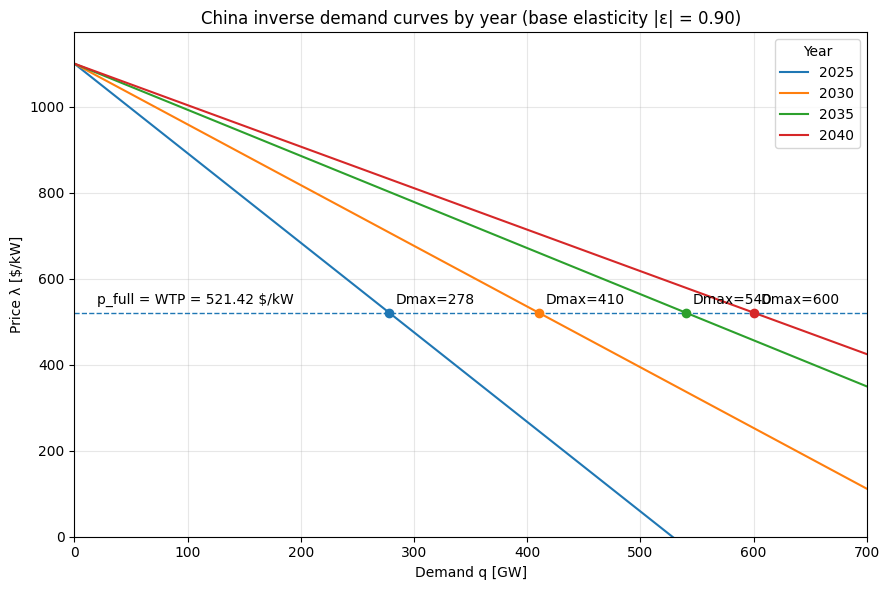
\includegraphics[width=0.9\textwidth]{output.png}
\caption{Calibrated inverse demand curves for China in 2025, 2030, 2035, and 2040 under the base elasticity case \(|\varepsilon|=0.90\). The dashed horizontal line indicates the full-demand threshold price \(p^{full}=WTP=521.42\ \$/\mathrm{kW}\). The marked points show that each yearly inverse demand curve passes through \(\bigl(D^{\max}_{t},\,WTP\bigr)\), i.e. full demand is served at the calibrated threshold price in every year.}
\label{fig:china_demand_curves}
\end{figure}








\section{Capacity Expansion and Fixed OPEX}

Regional capacity expansion costs are based on China as the baseline and scaled using regional cost multipliers:
\begin{equation}
CAPEX_{r,v} = m_r \cdot CAPEX^{ch}_{v},
\end{equation}
where $v$ denotes the PV manufacturing stage and $m_r$ the regional multiplier.

Fixed annual OPEX is assumed to equal 5\% of CAPEX:
\begin{equation}
OPEX_{r,v} = 0.05 \cdot CAPEX_{r,v}.
\end{equation}

\begin{table}[htbp]
\centering
\caption{Regional capacity expansion costs (CAPEX) and fixed operational costs (OPEX) across the full PV value chain.}
\label{tab:capex_opex_full_chain}
\begin{tabular}{l c r r r r r}
\toprule
\textbf{Region} & \textbf{Multiplier} & \textbf{Poly} & \textbf{Wafer} & \textbf{Cell} & \textbf{Module} & \textbf{Total} \\
\midrule
\multicolumn{7}{c}{\textbf{CAPEX [Million USD / GW]}} \\
\midrule
ch   & 1.00x & 70.0  & 100.0 & 180.0 & 50.0  & 400.0 \\
apac & 1.15x & 80.5  & 115.0 & 207.0 & 57.5  & 460.0 \\
row  & 2.50x & 175.0 & 250.0 & 450.0 & 125.0 & 1000.0 \\
af   & 3.00x & 210.0 & 300.0 & 540.0 & 150.0 & 1200.0 \\
eu   & 3.50x & 245.0 & 350.0 & 630.0 & 175.0 & 1400.0 \\
us   & 3.50x & 245.0 & 350.0 & 630.0 & 175.0 & 1400.0 \\
\midrule
\multicolumn{7}{c}{\textbf{Fixed OPEX [Million USD / GW / Year]}} \\
\midrule
ch   & 1.00x & 3.5  & 5.0  & 9.0  & 2.5  & 20.0 \\
apac & 1.15x & 4.0  & 5.8  & 10.4 & 2.9  & 23.0 \\
row  & 2.50x & 8.8  & 12.5 & 22.5 & 6.3  & 50.0 \\
af   & 3.00x & 10.5 & 15.0 & 27.0 & 7.5  & 60.0 \\
eu   & 3.50x & 12.3 & 17.5 & 31.5 & 8.8  & 70.0 \\
us   & 3.50x & 12.3 & 17.5 & 31.5 & 8.8  & 70.0 \\
\bottomrule
\end{tabular}

\vspace{0.6em}
\footnotesize
Notes: China baseline CAPEX values are taken from the IEA Solar PV Global Supply Chains report \cite{iea_solar_supply_2022}. Regional multipliers are informed by IEA and SolarPower Europe reshoring estimates \cite{spe_reshoring_2024}. Fixed OPEX is set to 5\% of CAPEX, following IEA clean technology manufacturing assumptions \cite{iea_cleantech_2023}.
\end{table}















\newpage
\section{Forecast: Annual Solar PV Additions in the IEA STEPS / Main Case}

The basis for this dataset is formed by the current reports of the IEA \cite{iea_weo_2024, iea_renewables_2025}. The following table shows the parameterized addition rates for the EPEC model in the Stated Policies Scenario (STEPS) and Main Case, respectively.

\begin{table}[htpb]
\centering
\begin{tabular}{llrrrr}
\toprule
\textbf{Region} & \textbf{Abbreviation} & \textbf{2025} & \textbf{2030} & \textbf{2035} & \textbf{2040} \\
\midrule
China & \texttt{ch} & 280.0 & 350.0 & 333.0 & 316.0 \\
Rest of Asia & \texttt{roa} & 50.0 & 85.0 & 103.0 & 126.0 \\
European Union & \texttt{eu} & 75.0 & 90.0 & 95.0 & 99.0 \\
USA & \texttt{us} & 45.0 & 65.0 & 70.0 & 75.0 \\
Africa & \texttt{af} & 5.0 & 10.0 & 14.0 & 20.0 \\
Rest of World & \texttt{row} & 45.0 & 70.0 & 79.0 & 89.0 \\
\midrule
\textit{Global (Control)} & \textit{Total} & \textit{500.0} & \textit{670.0} & \textit{694.0} & \textit{725.0} \\
\bottomrule
\end{tabular}
\caption{Annual solar PV additions in GW/year (own derivation based on IEA \cite{iea_weo_2024, iea_renewables_2025})}
\label{tab:pv_demand}
\end{table}

\subsection{Methodology and Transparent Derivation}

\subsubsection{Mathematical Aggregation of the Regions \texttt{roa} and \texttt{row}}
To strictly exclude overlaps and double counting in the model, the regions were adjusted from a balance-sheet perspective as follows:

\begin{itemize}
    \item \textbf{Rest of Asia (\texttt{roa}):} The IEA often reports the entire Asia-Pacific region (APAC) in its macro data. China massively dominates this region (approx. 80--85\% of additions). The calculation is therefore: 
    \begin{equation}
    \text{roa} = \text{APAC}_{\text{total}} - \text{China}_{\text{total}}
    \end{equation}
    \textit{Classification of Australia:} Australia is assigned to the Asia-Pacific region in the IEA's macroeconomic framework. It is therefore necessarily included in the \texttt{roa} region, along with other markets such as India, the ASEAN states, Japan, and South Korea.
    
    \item \textbf{Rest of World (\texttt{row}):} This residual value captures all remaining global capacities (e.g., Latin America, MENA region, Eurasia). The calculation is:
    \begin{equation}
    \text{row} = \text{World}_{\text{total}} - (\text{ch} + \text{roa} + \text{eu} + \text{us} + \text{af})
    \end{equation}
\end{itemize}

\subsubsection{CAGR Derivation for 2035 and 2040}
For the years 2025 and 2030, the addition rates could be derived from the IEA data \cite{iea_renewables_2025}. For 2035 and 2040, the formula for the Compound Annual Growth Rate (CAGR) was applied, supported by the STEPS narratives of the WEO 2024 \cite{iea_weo_2024}:

\begin{equation}
\text{Additions}_t = \text{Additions}_{2030} \cdot (1 + \text{CAGR})^{t - 2030}
\end{equation}

The chosen CAGR values reflect the regional market dynamics:
\begin{itemize}
    \item \textbf{\texttt{ch} (-1.0\%):} Market saturation and grid bottlenecks slightly dampen absolute growth after 2030.
    \item \textbf{\texttt{roa} (+4.0\%):} Catch-up electricity demand in the Asia-Pacific region.
    \item \textbf{\texttt{eu} (+1.0\%) \& \texttt{us} (+1.5\%):} Stable markets; replacement investments and progressive electrification.
    \item \textbf{\texttt{af} (+7.0\%):} Strongest relative growth due to microgrids and falling levelized costs of electricity (LCOE).
    \item \textbf{\texttt{row} (+2.5\%):} Moderate growth in the remaining global markets.
\end{itemize}


\subsubsection{Specific Sources and Referenced Chapters}
The extracted data points and underlying assumptions are based on the following specific sections of the cited IEA reports:

\begin{itemize}
    \item \textbf{IEA Renewables 2025 \cite{iea_renewables_2025}:} 
    The base year data as well as the short- and medium-term addition forecasts up to 2030 are taken from the \textit{Main Case}. The specific capacity values at the regional level are documented in the chapter \textit{"Electricity"} (particularly in the subchapters on solar PV and the regional forecast tables).
    
    \item \textbf{IEA World Energy Outlook 2024 \cite{iea_weo_2024}:} 
    The long-term market dynamics, saturation trends, and regional shifts for the period 2030 to 2040 are based on the \textit{Stated Policies Scenario (STEPS)}. The trends and baseline values used for this were taken from the chapter \textit{"Electricity"} (WEO standard chapter for power markets) as well as the comprehensive \textit{Data Annexes} (specifically the tables on "Electricity generation and capacity additions").
\end{itemize}




\bibliographystyle{plainnat}
\bibliography{literature}

\end{document}